\section{Ejercicio 10}

\subsection{Introducción}

Este ejercicio nos pide demostrar que el scheduler \textit{SchedEDF} no cumple con la propiedad enunciada en el ejercicio anterior cuando se presentan más de un núcleo de procesamiento.\\
Para simplificar el experimento trataremos el caso en el que sólo hay 2 núcleos de procesamiento disponibles, para el caso de más núcleos bastará con agregar tareas duplicadas como tanto núcleos adicionales se agreguen.\\
Además consideraremos que el scheduler tiene un costo por cambio de contexto igual a 1 y un costo por cambio de núcleo igual a 1.

\subsection{Demostración}
A fin de demostrar que dicha propiedad no se cumple bastará con encontrar un caso en cual \textit{SchedEDF} no ordene las tareas a utilizar el cpu de manera que todas puedan cumplir con su \textbf{deadline} y sin embargo exista un ordenamiento posible donde esto se pueda dar.\\
Consideremos el siguiente lote de tareas:

\begin{minipage}[t]{0.3\textwidth}
\begin{tarea}[H]
\begin{verbatim}
@0:
$15
TaskCPU 13
$7
TaskCPU 4
$10
TaskCPU 3
\end{verbatim}
\caption{Lote de 3 tareas}
\label{ej10-task}
\end{tarea}
\end{minipage}\\\\
En este lote la tarea \textit{$t_0$} tiene un \textbf{deadline} igual a 15 y un uso del cpu de 13 ciclos de reloj, la tarea \textit{$t_1$} tiene un \textbf{deadline} igual a 7 y un uso del cpu de 4 ciclos de reloj y la tarea \textit{$t_2$} tiene un \textbf{deadline} igual a 10 y un uso del cpu de 3 ciclos de reloj. Todas las tareas tienen un \textit{release time} igual a 0.\\\\
Ante esta situación \textit{SchedEDF} ejecutará primero \textit{$t_1$} y \textit{$t_2$} ya que tienen un \textbf{deadline} menor que \textit{$t_0$} y cuando alguna termine recién ejecutará \textit{$t_0$}, pero esta última no llegara a cumplir con su \textbf{deadline}.\\
A continuación se expone el diagrama de \textit{Gantt} para la situación descripta.

\begin{figure}[H]
\centering
\makebox[\textwidth][c]{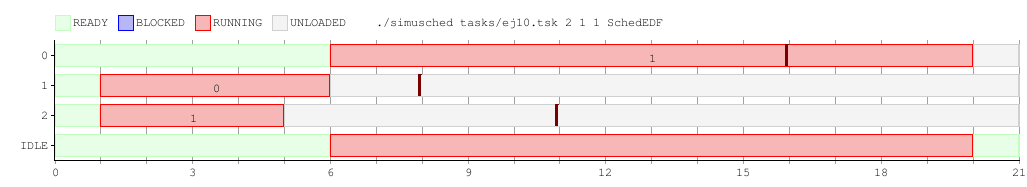
\includegraphics[width=1.2\textwidth]{graphics/ej10-01.png}}%
\caption{Lote de 3 tareas ejecutándose en \textit{SchedEDF}}
\label{ej10-edf-gantt}
\end{figure}

Sin embargo, si el scheduler hubiera elegido ejecutar primero \textit{$t_0$} y \textit{$t_1$} y al finalizar \textit{$t_1$} ejecutar \textit{$t_2$}, todas las tareas hubiesen cumplido con su \textbf{deadline}. Un scheduler que hubiese cumplido con dicho orden es por ejemplo \textit{SchedFCFS}.\\
A continuación se expone el diagrama de \textit{Gantt} para dicha situación.

\begin{figure}[h!t]
\centering
\makebox[\textwidth][c]{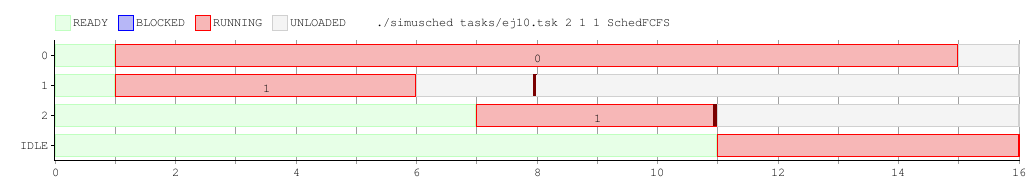
\includegraphics[width=1.2\textwidth]{graphics/ej10-02.png}}%
\caption{Lote de 3 tareas ejecutándose en \textit{SchedFCFS}}
\label{ej10-fcfs-gantt}
\end{figure}

\subsection{Conclusión}
 
Como puede observarse en el diagrama de \textit{Gantt} de la figura~\ref{ej10-edf-gantt}, dado el lote de tareas~\ref{ej10-task}, \textit{SchedEDF} no elige un ordenamiento óptimo por lo cual todas las tareas no llegan a cumplir su \textbf{deadline}.\\
Dicho ordenamiento existe y es posible, tal cual lo demuestra el diagrama de \textit{Gantt} de la figura~\ref{ej10-fcfs-gantt}, por lo tanto concluimos que el scheduler \textit{SchedEDF} no cumple con la propiedad enunciada en el ejercicio anterior cuando existe más de un núcleo de procesamiento.
